\chapter{Lavoro, Energia e Momenti}
L'obbiettivo di questo capitolo è quello di definire il lavoro e l'energia, e di stabilire la loro relazione, andando anche ad analizzare il concetto di momento ed analizzando alcuni esempi pratici e problemi di fisica.

\section{Lavoro}
    Il lavoro $W$ è definito come l'integrale in un certo percorso $\gamma$ nel quale la forza $\vec{F}$ agisce su un corpo di massa $m$:
    \begin{equation}
        W \stackrel{\text{def}}{=} \int_{\gamma} \vec{F} \cdot d\vec{l}
    \end{equation}
    dove $d\vec{l}$ è un elemento infinitesimo del percorso $\gamma$ e $\cdot$ indica il prodotto scalare. Il lavoro è una grandezza scalare, quindi non ha direzione, ma ha un valore numerico che può essere positivo o negativo a seconda della direzione della forza rispetto al movimento del corpo.\newline
    Prendiamo in considerazione una forza $\vec{F}$ applicata nella direzione $d$ di un corpo di massa $m$ appoggiato su un piano orizzontale, e che si muove di una distanza $d$ lungo la direzione della forza. Il lavoro compiuto dalla forza $\vec{F}$ è dato da:
    $$
        \begin{aligned}
            W_{Fd} =& \int_{\gamma} \vec{F} \cdot d\vec{l}\\
            =& \int_{\gamma} F\hat{x}\cdot (dx \hat{x})\\
            =& \int_{0}^{d} F dx\\
            =& Fd \qquad [N\cdot m] = [J]
        \end{aligned}
    $$
    dove $F$ è la forza applicata, $d$ è la distanza percorsa dal corpo e $\hat{x}$ è il versore della direzione della forza. Il lavoro compiuto dalla forza $\vec{F}$ è quindi dato dal prodotto della forza per la distanza percorsa dal corpo nella direzione della forza.\newline
    Ora se la forza applicata non fosse parallela alla direzione del movimento, ma formasse un angolo $\theta$ con la direzione del movimento, il lavoro compiuto dalla forza $\vec{F}$ sarebbe dato da:
    $$
        \begin{aligned}
            W_{Fd} =& \int_{\gamma} \vec{F} \cdot d\vec{l}\\
            =& \int_{\gamma} F\hat{l}\cdot (d\vec{x})\\
            =& Fd(\hat{l}\cdot \hat{x})\\
            =& Fd\cos(\theta)
        \end{aligned}
    $$
    Da questa ultima possiamo distinguere tre casi:
    \begin{itemize}
        \item $0\leq \theta < \frac{\pi}2 \Rightarrow \cos \theta > 0$ Allora $W_{Fd} > 0$ e la forza $\vec{F}$ compie \textbf{Lavoro Motore} sul corpo.
        \item $\theta = \frac{\pi}2 \Rightarrow \cos \theta = 0$ Allora $W_{Fd} = 0$ e la forza $\vec{F}$ non compie lavoro sul corpo.
        \item $\frac{\pi}2 < \theta \leq \pi \Rightarrow \cos \theta < 0$ Allora $W_{Fd} < 0$ e la forza $\vec{F}$ compie \textbf{Lavoro Frenante} sul corpo.
    \end{itemize}
    \subsubsection{Problema 1 - Massa che scivola su un piano inclinato}
        Consideriamo una massa $m$ che scivola su un piano inclinato di angolo $\alpha$ rispetto all'orizzontale.\newline
        In questo caso la forza peso $\vec{P}$ esegue un lavoro positivo sulla massa, non consideriamo al momento l'attrito, quindi la forza peso che spinge la massa lungo il piano inclinato è data da:
        $$
            \vec{P} = m\vec{g}
        $$
        ma in quanto l'asse $z$ sul quale è applicata la forza peso e misurata l'altezza $h$ forma un angolo $\theta=\pi-\left(\frac{\pi}2-\alpha\right) = \frac{pi}{2}+\alpha$ con l'asse $x$, il l'infinitesimo lavoro compiuto dalla forza peso $\vec{P}$ è dato da:
        $$
            \begin{aligned}
                dw=& F_{P} \cdot \hat{l} \\
                =& -mg\hat{z} \cdot (di\cdot \hat{i})\\
                =& -mg\ di\ \hat{z} \cdot \hat{i}\\
                =& -mg\ di\ \cos(\theta)\\
                =& +mg\ di\ \sin(\alpha)\\
                =& P_{\parallel} di\\
            \end{aligned}
        $$
        dove $P_{\parallel}$ è la componente della forza peso $\vec{P}$ lungo il piano inclinato. Dunque il lavoro compiuto dalla forza peso $\vec{P}$ è dato da:
        $$
            \begin{aligned}
                W_{P} =& \int_{\gamma} P_{\parallel} dw\\
                =& mg\sin(\alpha) L\\
                =& mg h
            \end{aligned}
        $$
        dove $L$ è la lunghezza del piano inclinato e $h$ è l'altezza della massa rispetto al piano orizzontale, abbiamo sostituito $L$ con $h$ in quanto la lunghezza del piano inclinato moltiplicata per il seno dell'angolo $\alpha$, che è l'opposto del triangolo rettangolo, è uguale all'altezza $h$ della massa rispetto al piano orizzontale. Quindi il lavoro compiuto dalla forza peso $\vec{P}$ sulla massa $m$ è dato dal prodotto della forza peso per l'altezza della massa rispetto al piano orizzontale, dunque il lavoro compiuto dalla forza peso $\vec{P}$ sulla massa $m$ è \underline{indipendente} dall'angolo $\alpha$ del piano inclinato, ma dipende esclusivamente dall'altezza $h$ della massa rispetto al piano orizzontale.
        \begin{figure}[H]
            \centering
            \begin{subfigure}[b]{0.45\textwidth}
                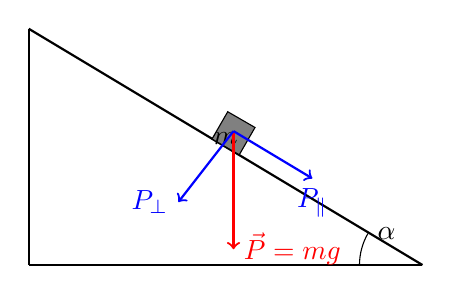
\begin{tikzpicture}
                    % Disegna il piano inclinato con angolo retto in basso a sinistra
                    \draw[thick] (0,0) -- (5,0);
                    \draw[thick] (0,0) -- (0,3);
                    \draw[thick] (0,3) -- (5,0);
                    
                    % Massa appoggiata in diagonale sul piano inclinato
                    \draw[fill=gray, rotate around={-30:(2.5,1.5)}] (2.3,1.5) rectangle (2.7,1.9);
                    \node at (2.5,1.6) {$m$};
                    
                    % Angolo
                    \draw (4.2,0) arc (180:150:0.8) node[right] {$\alpha$};
                    
                    % Forza peso
                    \draw[->, thick, red] (2.6,1.7) --++ (0,-1.5) node[right] {$\vec{P} = mg$};
                    
                    % Componenti della forza peso
                    \draw[->, thick, blue] (2.6,1.7) --++ (1,-0.6) node[below] {$P_{\parallel}$};
                    \draw[->, thick, blue] (2.6,1.7) --++ (-0.7,-0.9) node[left] {$P_{\perp}$};
                \end{tikzpicture}
            \end{subfigure}
            \begin{subfigure}[b]{0.45\textwidth}
                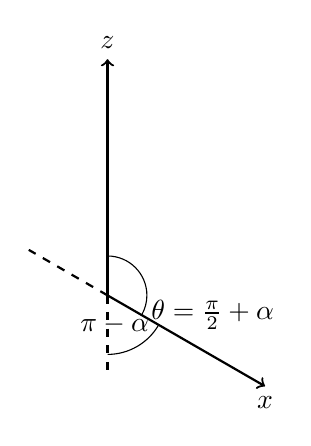
\begin{tikzpicture}
                    % Asse di riferimento inclinato
                    \draw[thick,->] (0,0) -- (0,3) node[above] {$z$};
                    \draw[thick,->] (0,0) -- (2,-1.154) node[below] {$x$};
                    \draw[thick, dashed] (0,0) -- (0,-1);
                    \draw[thick, dashed] (0,0) -- (-1,0.5777);
                    \draw (0,0.5) arc (90:-30:0.5) node[right] {$\theta = \frac{\pi}{2}+\alpha$};
                    \draw (0,-0.75) arc (270:330:0.75) node[left] {$\pi-\alpha$};
                \end{tikzpicture}
            \end{subfigure}
            \caption{Massa su piano inclinato e rappresentazione del sistema di riferimento.}
        \end{figure}
    \subsubsection{Problema 2 - Massa su piano inclinato con attrito}
        Consideriamo una massa $m$ che scivola su un piano inclinato di angolo $\alpha$ rispetto all'orizzontale, e che è soggetta ad un attrito dinamico di coefficiente $\mu_d$.\newline
        In questo caso la forza peso $\vec{P}$ esegue un lavoro positivo sulla massa, mentre la forza di attrito $\vec{F}_{attr}$ esegue un lavoro negativo sulla massa. La forza di attrito è data da:
        $$
            \vec{A_d}= -\mu_d \left|\vec{N}\right|\hat{v}
        $$
        dove $\vec{N}$ è la forza normale, che in questo caso è data dalla componente della forza peso $\vec{P}$ perpendicolare al piano inclinato, e $\hat{v}$ è il versore della direzione del movimento della massa. L'infinitesimo lavoro compiuto dalla forza di attrito $\vec{A_d}$ è dato da:
        $$
            \begin{aligned}
                dw=& F_{A_d} \cdot d\hat{l} \\
                =& -\mu_d \left|\vec{N}\right|\hat{v} \cdot (dl\cdot \hat{v})\\
                =& -\mu_d mg\cos (\alpha) dl\\
            \end{aligned}
        $$
        dove $dl$ è l'infinitesimo spostamento della massa lungo il piano inclinato. Dunque il lavoro compiuto dalla forza di attrito $W_{A_d}$ è dato da:
        $$
            \begin{aligned}
                W_{A_d} =& \int_{\gamma} A_d dw\\
                =& -\mu_d mg\cos(\alpha)\int_0^L dl\\
                =& -\mu_d mg\cos(\alpha) L\\
            \end{aligned}
        $$
        dove $L$ è la lunghezza del piano inclinato. Quindi il lavoro compiuto dalla forza di attrito $\vec{A_d}$ sulla massa $m$ è dato dal prodotto della forza di attrito per la lunghezza del piano inclinato, dunque il lavoro compiuto dalla forza di attrito $\vec{A_d}$ sulla massa $m$ è \underline{dipendente}, al contrario della forza peso $\vec{P}$, dall'angolo $\alpha$ del piano inclinato.
\section{Teorema delle forze vive}
    Il teorema delle forze vive, nei sistemi inerziali, afferma che la somma dei lavori compiuti dalle forze agenti su un corpo è uguale alla variazione dell'energia cinetica del corpo stesso. In formula:
    \begin{equation}
        \sum W_{i} = \Delta K
    \end{equation}
    Questo è dimostrabile in quanto
    $$
        \begin{aligned}
            \vec{F} =& m\vec{a} \qquad & \text{Seconda Legge di Newton}\\
            =& m\frac{d\vec{v}}{dt} \qquad & \text{Definizione di accelerazione}\\
            \vec{F}d\vec{s} =& m\frac{d\vec{v}}{dt}d\vec{s}\\
            =& m(d\vec{v})\frac{d\vec{s}}{dt}\\
            =& m(d\vec{v})\vec{v}\\
        \end{aligned}
    $$
    dunque da questa otteniamo che la somma delle forze agenti su un corpo moltiplicata per l'infinitesimo spostamento del corpo è uguale alla variazione della velocità del corpo moltiplicata per la velocità del corpo stesso. Possiamo però esprimere $\vec{v}d\vec{v}$ come:
    $$
        \begin{aligned}
            \vec{v}d\vec{v} =& v_xdv_x + v_ydv_y + v_zdv_z\\
            =&d\left[\frac{v_x^2}2\right] + d\left[\frac{v_y^2}2\right] + d\left[\frac{v_z^2}2\right]\\
            =& \frac12d\left[v_x^2 + v_y^2 + v_z^2\right]\\
            =& \frac12d\left[v^2\right]\\
        \end{aligned}
    $$
    andando quindi a unire le due equazioni otteniamo:
    $$
        \begin{aligned}
            \vec{F}d\vec{s} =& \frac12m d\left[v^2\right]\\
            \downarrow & \qquad \text{Integrando}\\
            \int_i^f dw =& \int_i^f \frac12m d\left[v^2\right]
        \end{aligned}
    $$
    e dunque per descrivere il lavoro esercitato su un corpo da una forza $\vec{F}$ dal punto $i$ al punto $f$ otteniamo:
    \begin{align}
        W_{F,i\to f} =& \frac12mv_f^2-\frac12mv_i^2 = \Delta E_K \\
        E_K \stackrel{def}{=}& \frac12mv^2
    \end{align}
    dove $E_K$ è l'energia cinetica del corpo, che è definita come la metà del prodotto della massa del corpo per il quadrato della sua velocità. L'energia cinetica è una grandezza scalare, quindi non ha direzione, ma ha un valore numerico che può essere positivo o negativo a seconda della direzione della velocità del corpo, questa è espressa in Joule $[J]$ ed ha dunque dimensionalità del lavoro $[J] = [N\cdot m] = [kg\cdot m^2/s^2]$.
\section{Forze Conservative}
    Le forze conservative sono forze che compiono lavoro indipendentemente dal percorso seguito dal corpo, ma solo dalla posizione iniziale e finale del corpo stesso, ad esempio la forza peso $\vec{P}$ è una forza conservativa, mentre la forza di attrito $\vec{A_d}$ non lo è. Visto che dipendono solo dalla posizione iniziale e finale del corpo, possiamo scrivere le seguenti relazioni:
    \begin{align}
        \vec{F}|_{W_{i\to f}} =& \int_i^f \vec{F}\cdot d\vec{s} \label{eq:forzaConservativa}
    \end{align}
    Ovvero il lavoro compiuto dalla forza $\vec{F}$ su un corpo che si sposta da una posizione $i$ ad una posizione $f$ è indipendente dal percorso ma solo dalla posizione iniziale e finale del corpo stesso.\newline
    Questo ci permette di scrivere:
    \begin{align}
        \oint \vec{F}\cdot d\vec{s} =& 0 \label{eq:forzaConservativa2}
    \end{align}
    considerando dunque l'Equazione \ref{eq:forzaConservativa} e l'Equazione \ref{eq:forzaConservativa2} le quali sono equivalenti e semplicemente dimostrabili usando le proprietà degli integrali, possiamo definire il lavoro di una forza conservativa come:
    \begin{align}
        W_{F,i\to f} =& \mathcal{F} \label{eq:forzaConservativa3}
    \end{align}
    Se l'Equazione \ref{eq:forzaConservativa3} non risultasse verificata allora la forza $\vec{F}$ non sarebbe conservativa, e quindi il lavoro compiuto dalla forza $\vec{F}$ su un corpo che si sposta da una posizione $i$ ad una posizione $f$ dipenderebbe dal percorso seguito dal corpo stesso.
\section{Energia Potenziale}
    \label{subsec:energiaPotenziale}
    Prendiamo in considerazione una forza conservativa $\vec{F}$, dunque il lavoro compiuto dalla forza $\vec{F}$ su un corpo che si sposta da una posizione $i$ ad una posizione $f$ è indipendente dal percorso ma solo dalla posizione iniziale e finale del corpo stesso. Fissiamo ora il punto $i\rightarrow O$ come punto di originario, e il punto $f\rightarrow P$ come punto finale del corpo stesso, quindi possiamo scrivere:
    \begin{equation}
        E_{\rho}(x,y,z)=E_{\rho,P}=-\int_{O}^{P} \vec{F}\cdot d\vec{s} \label{eq:energiaPotenziale}
    \end{equation}
    abbiamo dunque definito l'\textbf{energia potenziale} $E_{\rho}$ del punto $P$ come il lavoro compiuto dalla forza $\vec{F}$ su un corpo che si sposta dal punto $O$ al punto $P$. La funzione \ref{eq:energiaPotenziale} è definita \textbf{funzione potenziale} della forza $\vec{F}$, questa descrive l'energia potenziale del corpo in funzione della sua posizione nello spazio ($x,y,z$). L'energia potenziale è una grandezza scalare, quindi non ha direzione, ma ha un valore numerico che può essere positivo o negativo a seconda della posizione del corpo nello spazio. L'energia potenziale è espressa in Joule $[J]$ ed ha dunque dimensionalità del lavoro $[J] = [N\cdot m] = [kg\cdot m^2/s^2]$.
    \paragraph{Proprietà} Se al posto di considerare il punto $O$ come punto di origine, considerassimo un altro punto $A$ ed un altro punto $B$, allora il lavoro compiuto dalla forza $\vec{F}$ su un corpo che si sposta dal punto $A$ al punto $B$ sarebbe dato da:
    $$
        \begin{aligned}
            W_{F,A\to B} =& \int_{A}^{B} \vec{F}\cdot d\vec{s}\\
            =& \int_{A}^{O} \vec{F}\cdot d\vec{s} + \int_{O}^{B} \vec{F}\cdot d\vec{s}\\
            =& -\int_{O}^{A} \vec{F}\cdot d\vec{s} - \int_{O}^{B} \vec{F}\cdot d\vec{s}
        \end{aligned}
    $$
    Da questa ricaviamo che:
    \begin{equation}
        W_{F,A\to B}=E_{\rho, A} - E_{\rho,B} = \Delta E_{\rho} \label{eq:energiaPotenziale2}
    \end{equation}
    Da notare come nel calcolo dell'energia potenziale per qualunque punto $O$ scelto come origine non influisce sul risultato dell'Equazione \ref{eq:energiaPotenziale2}. Anche in questa si nota come per le forze conservative se il punto di inizio e il punto di fine sono gli stessi, e si vuole quindi calcolare il lavoro compiuto, questo risulterà essere nullo per l'Equazione \ref{eq:forzaConservativa2}, ciò in quanto se considerassimo un qualsiasi punto intermedio $M$ nel percorso che inizia e termina nello stesso punto $A$ allora ``quello che guadagna il corpo nel percorso $A\to M$ lo perde nel percorso $M\to A$'', dunque l+integrale chiuso risulterebbe essere nullo.
    \subsubsection{Energia potenziale forza peso}
        Applicando l'Equazione \ref{eq:energiaPotenziale} alla forza peso $\vec{P}$, otteniamo:
        \begin{equation}
            E_{\rho, P} = mgz.
        \end{equation}
        Dove $z$ è l'altezza del corpo rispetto al piano orizzontale, e $m$ è la massa del corpo. L'energia potenziale della forza peso è quindi direttamente proporzionale all'altezza del corpo rispetto al piano orizzontale, e alla massa del corpo stesso. Il segno dell'energia potenziale della forza peso è positivo, in quanto la forza peso compie lavoro positivo sul corpo quando questo si sposta verso l'alto, e negativo quando il corpo si sposta verso il basso.\newline
        \textbf{N.B. \ref{lez:31-03-2025}}
\section{Conservazione dell'energia meccanica}
    \label{subsec:conservazioneEnergiaMeccanica}
    Nell'ipotesi che su una massa non agiscano forze dissipative, allora dato che valgono contemporaneamente le Equazioni \ref{eq:forzaConservativa} e \ref{eq:energiaPotenziale2}, possiamo combinarle e scrivere:
    \begin{align}
        W =& \Delta E_K = E_{K,B} - E_{K,A} \nonumber\\
        W =& -\Delta E_{\rho} = E_{\rho,A} - E_{\rho,B} \nonumber\\
        E_{k,A} + E_{\rho,A} =& E_{k,B} + E_{\rho,B} 
    \end{align}
    Dunque se non agiscono forze dissipative: ``La somma dell'energia cinetica e dell'energia potenziale di un corpo è costante''. Il che è il principio di conservazione dell'\textbf{energia meccanica}, che afferma che l'energia meccanica totale di un corpo è costante se non agiscono forze dissipative sul corpo stesso. \newline
    Se in un corpo agiscono allo stesso tempo forze conservative e forze dissipative, allora la somma dell'energia cinetica e dell'energia potenziale del corpo non è costante, ma varia nel tempo in funzione del lavoro compiuto dalle forze dissipative. Dunque
    \begin{align*}
        W =& W_{c} + W_{nc} &= E_{k,B} - E_{k,A}\\
        & E_{\rho,A} - E_{\rho,B} + W_{nc} &= E_{k,B} - E_{k,A}\\
        W_{nc} =& (E_{k,B} + E_{\rho,B}) - (E_{k,A} + E_{\rho,A})&\\
        =& E_{m,B} - E_{m,A}\\
    \end{align*}
    Dove $W_{nc}$ è il lavoro compiuto dalle forze non conservative, $E_{m}$ è l'energia meccanica totale del corpo, e $E_{m,A}$ e $E_{m,B}$ sono le energie meccaniche totali del corpo nei punti $A$ e $B$ rispettivamente. In sostanza se agiscono forze non conservative sul corpo, allora la somma dell'energia cinetica e dell'energia potenziale del corpo varia nel tempo in funzione del lavoro compiuto dalle forze non conservative.\newline
    \textbf{N.B. \ref{lez:31-03-2025}}
\section{Potenza}
    La potenza è definita come il lavoro in un certo lasso di tempo, dunque:
    \begin{equation}
        \overline{P}=\frac{W}{\Delta t}
    \end{equation}
    Questa è definita come la potenza media del lavoro $W$ nel tempo $\Delta t$, se al posto di questo vogliamo conoscere la ``potenza istantanea'', con un abuso di notazione andando a prendere l'infinitesimo lavoro $dW$ che non ha un vero e proprio senso, scriviamo:
    \begin{equation}
        P=\frac{dW}{dt}
    \end{equation}
    dimensionalmente l'unità di misura della potenza è il Watt ($\operatorname{W}$) che è quindi definita come
    \begin{equation*}
        [P]=\left[\frac{E}{T}\right]=\left[F\cdot\frac{L}{T}\right]=\left[M\cdot\frac{L}{T^2}\cdot\frac{L}{T}\right]=\left[F\cdot V\right]
    \end{equation*}